\newpage
\section{Objectif : Responsable des stocks}
Le responsable des stocks cherche à minimiser le nombre de de produits dans
son stock sous les contraintes définies précedemment.

\subsection{Modélisation}
Soit $Stock(n_{i})$ le nombre d'unités de stock nécessaires pour stocker les
produits fabriqués et la matière première nécessaire. Cette fonction est la
somme des produits fabriqués à laquelle on ajoute la quantité de matières
premières nécessaire à la fabrication.

On suppose qu'un produit frabriqué correspond à une unité de stock.

On a ainsi la formule suivante, où $n_{i}$ est la quantité de produit usiné
(pour chaque produit $i$), et $Q_{j,i}$ est la quantité de matière première
par produit pour chaque produit $i$ et chaque matière première $j$.

\begin{equation}
	Stock(n) = \sum_{i} (n_{i} + n_{i} \times \sum_{j} Q_{j,i})
\end{equation}

La représentation matricielle de cette fonction sera alors :

\begin{equation}
	M_S = \begin{pmatrix}
		1 & 1 & 1 & 1 & 1 & 1
	\end{pmatrix} + (
	\begin{pmatrix}
		1 & 1 & 1
	\end{pmatrix}
	\times Q)
\end{equation}

Le résultat trivial est :
\begin{pmatrix}
	0 \\ 0 \\ 0 \\ 0 \\ 0 \\ 0
\end{pmatrix}

En effet, en l'absence de production, aucun stock n'est nécessaire. Ce résultat
n'est pas satisfaisant. Nous allons donc nous intéresser à un second critère :
les bénéfices de l'entreprise. Pour ce faire, nous allons nous intéresser aux
valeurs obtenues en imposant un minimum de bénéfices. En réalisant les calculs
sur plusieurs échelons, on obtient un résultat linéaire par morceaux. Le
raisonement adopté est similaire à celui développé dans la section
\ref{sec:monocrit_resp_com}.

\begin{figure}[h!]
	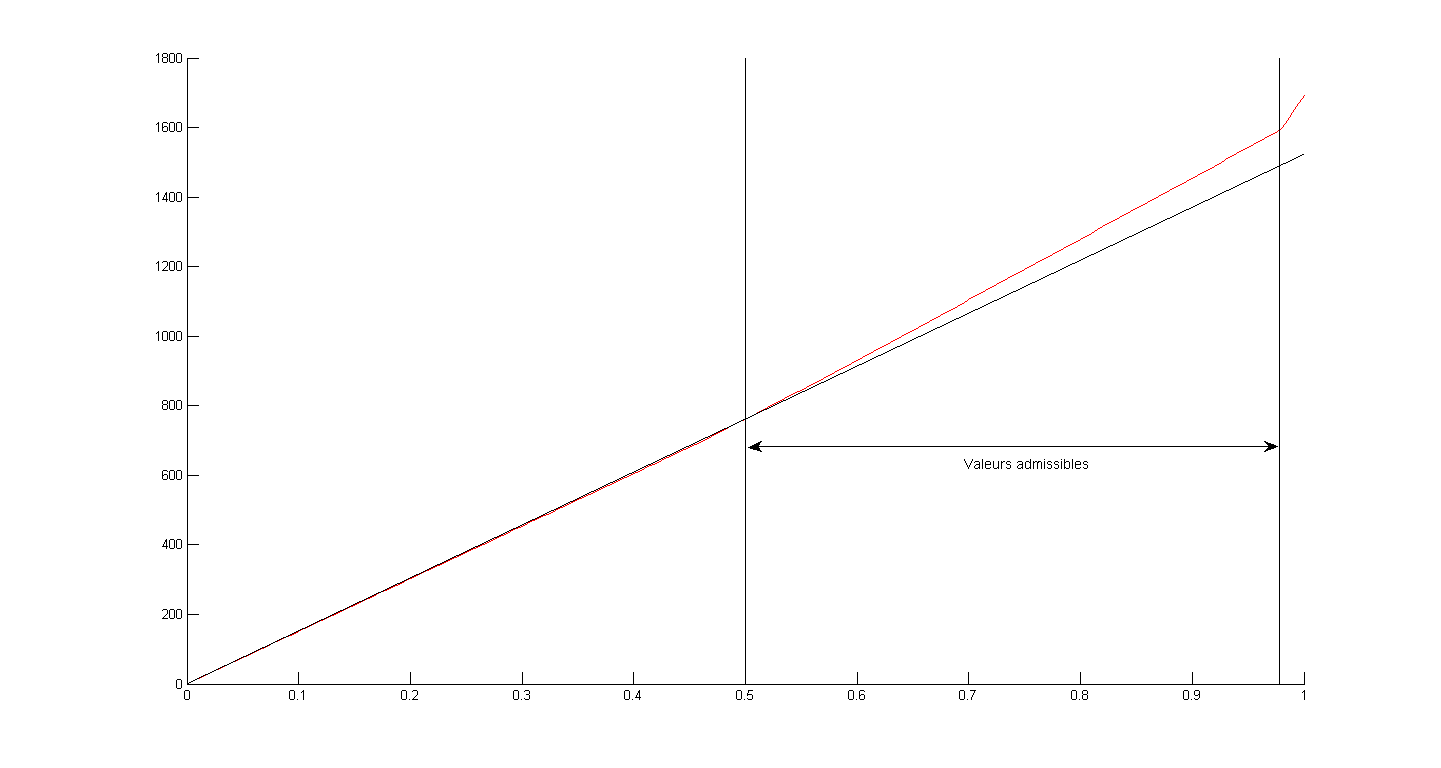
\includegraphics[width=\textwidth]{SourcesMatlab/graphe_resp_stocks.png}
	\caption{Graphe de l'évolution des stocks en fonction du bénéfice}
\end{figure}


\subsection{Décisions}
De nombreuses valeurs sont équivalentes et ne peuvent être départagées selon des
critères mathématiques. Les choix possibles se situent dans le deuxième morceau
de courbe : en dessous, les bénéfices sont trop bas, au dessus, les besoins de
stockage augmentent beaucoup plus que les bénéfices.

On a donc une valeur comprise entre 50\% et 98\% de bénéfices. Pour 75\% du
bénéfice maximum, on obtient le nombre de produits suivants :

\begin{pmatrix}
1,91903382074088 \times 10^{-10} \\
2,63753463514149 \times 10^{-10} \\ 
1,89174897968769 \times 10^{-10} \\
1,23691279441118 \times 10^{-10} \\ 
124,634235411818 \\
142,146305832495
\end{pmatrix}
pour une quantité d'unités en stock de 1191,75640039347.



